\PassOptionsToPackage{unicode=true}{hyperref} % options for packages loaded elsewhere
\PassOptionsToPackage{hyphens}{url}
%
\documentclass[12pt,a4paperpaper,]{tufte-book}
\usepackage{lmodern}
\usepackage{amssymb,amsmath}
\usepackage{ifxetex,ifluatex}
\usepackage{fixltx2e} % provides \textsubscript
\ifnum 0\ifxetex 1\fi\ifluatex 1\fi=0 % if pdftex
  \usepackage[T1]{fontenc}
  \usepackage[utf8]{inputenc}
  \usepackage{textcomp} % provides euro and other symbols
\else % if luatex or xelatex
  \usepackage{unicode-math}
  \defaultfontfeatures{Ligatures=TeX,Scale=MatchLowercase}
\fi
% use upquote if available, for straight quotes in verbatim environments
\IfFileExists{upquote.sty}{\usepackage{upquote}}{}
% use microtype if available
\IfFileExists{microtype.sty}{%
\usepackage[]{microtype}
\UseMicrotypeSet[protrusion]{basicmath} % disable protrusion for tt fonts
}{}
\IfFileExists{parskip.sty}{%
\usepackage{parskip}
}{% else
\setlength{\parindent}{0pt}
\setlength{\parskip}{6pt plus 2pt minus 1pt}
}
\usepackage{hyperref}
\hypersetup{
            pdftitle={Emergent Collective Properties in Societies of Neural Networks},
            pdfauthor={Lucas Silva Simões},
            pdfborder={0 0 0},
            breaklinks=true}
\urlstyle{same}  % don't use monospace font for urls
\usepackage{graphicx,grffile}
\makeatletter
\def\maxwidth{\ifdim\Gin@nat@width>\linewidth\linewidth\else\Gin@nat@width\fi}
\def\maxheight{\ifdim\Gin@nat@height>\textheight\textheight\else\Gin@nat@height\fi}
\makeatother
% Scale images if necessary, so that they will not overflow the page
% margins by default, and it is still possible to overwrite the defaults
% using explicit options in \includegraphics[width, height, ...]{}
\setkeys{Gin}{width=\maxwidth,height=\maxheight,keepaspectratio}
\setlength{\emergencystretch}{3em}  % prevent overfull lines
\providecommand{\tightlist}{%
  \setlength{\itemsep}{0pt}\setlength{\parskip}{0pt}}
\setcounter{secnumdepth}{5}
% Redefines (sub)paragraphs to behave more like sections
\ifx\paragraph\undefined\else
\let\oldparagraph\paragraph
\renewcommand{\paragraph}[1]{\oldparagraph{#1}\mbox{}}
\fi
\ifx\subparagraph\undefined\else
\let\oldsubparagraph\subparagraph
\renewcommand{\subparagraph}[1]{\oldsubparagraph{#1}\mbox{}}
\fi

% set default figure placement to htbp
\makeatletter
\def\fps@figure{htbp}
\makeatother

\makeatletter
\@ifpackageloaded{subfig}{}{\usepackage{subfig}}
\@ifpackageloaded{caption}{}{\usepackage{caption}}
\captionsetup[subfloat]{margin=0.5em}
\AtBeginDocument{%
\renewcommand*\figurename{Figure}
\renewcommand*\tablename{Table}
}
\AtBeginDocument{%
\renewcommand*\listfigurename{List of Figures}
\renewcommand*\listtablename{List of Tables}
}
\@ifpackageloaded{float}{}{\usepackage{float}}
\floatstyle{ruled}
\@ifundefined{c@chapter}{\newfloat{codelisting}{h}{lop}}{\newfloat{codelisting}{h}{lop}[chapter]}
\floatname{codelisting}{Listing}
\newcommand*\listoflistings{\listof{codelisting}{List of Listings}}
\makeatother

\title{Emergent Collective Properties in Societies of Neural Networks}
\author{Lucas Silva Simões}
\date{2016-2 and 2017-1}

\begin{document}
\maketitle

{
\setcounter{tocdepth}{3}
\tableofcontents
}
\hypertarget{sec:summary}{%
\section{Summary}\label{sec:summary}}

We model a society of agents who interact in pairs by exchanging for/against opinions about issues using a perceptron algorithm. Employing a maximum entropy analysis one can describe the interacting pair as a dynamics along the gradient of the logarithm of the evidence. This permits introducing an energy like quantity and an approximate global hamiltonian. Knowledge of the expected value of the hamiltonian is relevant information for the state of the society, inducing a canonical distribution by maximum entropy. We study the phase diagram of the society using a mean field approximation which indicate a phase transitions separating ordered and disordered phases depending on the society parameters.

\hypertarget{sec:bayeslearn}{%
\section{Bayesian Machine Update Learning}\label{sec:bayeslearn}}

Consider a machine prepared to work with a fixed (\emph{hardcoded}) model \(\mathcal{M}\) which depends on some internal variables \(\mathbf{x}\). Such machine is presented with examples \(\mathcal{D}_t = \left\{ (\xi_\mu, \sigma_\mu)_{\mu=1}^t \right\}\) and seeks to update its knowledge about \(\mathbf{x}\) in such a way to describe correctly (with \(\mathcal{M}\)) the received examples while still improving its ability to predict future inputs (also known as capability of \emph{generalization}).

That machine needs to somehow codify which values of \(\mathbf{x}\) are more appropriate to the classification task being learned. As this is an incomplete information situation (that is, we do not have full access to the optimal parameters \(\hat{\mathbf{x}}\)), we use probability theory tools to describe the plausibility (or beliefs) the machine attributes - through its mechanical-logical-electronic processes - to each value of \(\mathbf{x}\). This we call the distribution \(Q(\mathbf{x})\).

By means of practicality we are going to consider that the distribution \(Q(\mathbf{x})\) belongs to some \emph{parametric family} of probability distributions. That is, there is a set of conditions (from now on called \textbf{generators}) satisfied by and, more than that, \emph{defining} the utilized distribution:

\[ \exists\ \{F_a(\mathbf{x})\}_{a=1}^G\ \ \text{such that} \ \ \mathbb{E}_Q[F_a] = \eta_a \]

The technological (and evolutionary) justification supporting the choice of a parametric family comes from noticing that the machine's memory (or the animal's brain, in a biology analogy) is limited and thus can only store a finite amount of information usable by its processing. Therefore it is viable that we imagine a numberless of different machines with different architectures (which differ on the parametric family used) and then compare their performances in different settings.

In possession of the generators we can do Maximum Entropy and obtain:

\[Q(\mathbf{x}) = P(\mathbf{x}|\theta) = \frac1\zeta \exp\left(- \sum_{a=1}^G \theta_a F_a(\mathbf{x}) \right)\]

where \(\zeta = \int \mathrm{d}\mathbf{x}\ \exp\left(- \sum_{a=1}^G \theta_a F_a(\mathbf{x})\right)\) is the normalization of the probability distribution \(Q\), also called the \textbf{partition function}. We calculate some identities that are going to be useful later on:

\[  \frac{\partial \log \zeta}{\partial \theta_b} = \frac1\zeta \frac{\partial \zeta}{\partial \theta_b} = \frac1\zeta \int \mathrm{d}\mathbf{x}\ (-F_b(\mathbf{x})) \mathrm{e}^{- \sum_a \theta_a F_a(\mathbf{x})} \]

\begin{equation} \qquad\therefore\ \frac{\partial \log \zeta}{\partial \theta_b} = - \eta_b \label{eq:ident1}\end{equation}

\[  \frac{\partial Q}{\partial \theta_b} = \frac1\zeta \mathrm{e}^{- \sum_a \theta_a F_a(\mathbf{x})} \left( -F_b(\mathbf{x})\right) +  \mathrm{e}^{- \sum_a \theta_a F_a(\mathbf{x})} \left( \frac{-1}{\zeta^2} \right) \frac{\partial \zeta}{\partial \theta_b} \]

\begin{equation} \qquad\therefore\ \frac{\partial Q}{\partial \theta_b} = [\eta_b - F_b(\mathbf{x})] Q \label{eq:ident2}\end{equation}

Knowing the probability distribution the machine attributes to the parameters of its interior model, we might calculate how it is that the ``knowledge'' of the machine will change when a new example is presented to it. Using Bayes' Theorem:

\[ P_{n+1}(\mathbf{x}) = P(\mathbf{x}| \mathcal{D}_{n+1}) = \frac{L_{n+1} Q_n}{Z_{n+1}} = \frac{P(\mathcal{D}_{n+1}| \mathbf{x})\ P(\mathbf{x}| \theta_n)}{\int \mathrm{d}\mathbf{x}\ P(\mathcal{D}_{n+1}| \mathbf{x})\ P(\mathbf{x}| \theta_n)}\]

Although this update is exact, it does not suit our needs since the new distribution \(P_{n+1}\) usually will not belong to the initial parametric family. We need an alternative step that takes into account the relevant data from Bayes' rule and remains with the same functional form as the prior.

To do that one can minimize the distance (maximize the entropy) between the distributions \(D_{KL}[Q_{n+1}||Q_n]\) while enforcing the expectation values of \(P_n\) with \(\mathbb{E}_{P_n}[F_a(\mathbf{x})] = \eta_a\). We want to minimize the following Lagrangian\footnote{Here we start using Einstein summation convention \[ x_a y^a \equiv \sum_a x_a y_a \]}:

\begin{align}
     \Lambda[P, Q, \{\Delta_a\}] = &\int \mathrm{d}\mathbf{x}\ Q_{n+1} \log\frac{Q_{n+1}}{Q_n} - \Delta^a \left[\int \mathrm{d}\mathbf{x}\ F_a Q_{n+1} - \eta_a \right] \\
    &\quad - \Delta_0 \left[ \int \mathrm{d}\mathbf{x}\ Q_{n+1} - 1 \right]
\end{align}

Since both \(Q_n\) and \(P_n\) are already fixed, one can only minimize the Lagrangian varying the posterior distribution \(Q_{n+1}\). Taking a functional derivative, one finds:

\[ \frac{\delta \Lambda}{\delta Q_{n+1}} = \int \mathrm{d}\mathbf{x}\ \delta Q_{n+1} \left[ \log Q_{n+1} + 1 - \log Q_n - \Delta^a F_a - \Delta_0 \right]\]

\begin{figure}
\hypertarget{fig:updateproject}{%
\centering
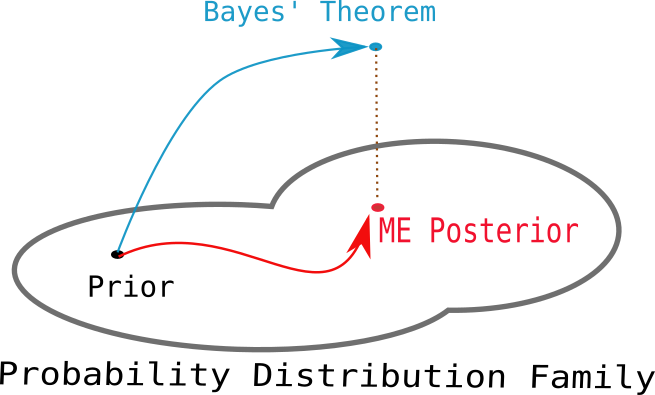
\includegraphics[width=0.55\textwidth,height=\textheight]{images/em-updateproject.png}
\caption{Schematic representation of the update procedure done to revise the distribution \(Q_n\). It goes as follows: one uses Bayes' Theorem (blue path) to get the new constraints and then updates the distribution through maximum entropy (red path), therefore minimizing the distance relative to the prior while enforcing the new expected values of the posterior.}\label{fig:updateproject}
}
\end{figure}

Equating this to zero, one finds the expression for the Maximum Entropy (ME) posterior:

\[Q_{n+1}(\mathbf{x}) = Q_n(\mathbf{x})\ \mathrm{e}^{-1 + \Delta_0 + \Delta^a F_a} = \frac{1}{\zeta_{n+1}} \exp\left(- \sum_{a=1}^G \theta_a^{n+1} F_a(\mathbf{x}) \right)\]

where \(\theta^{n+1}_a = \theta^n_a + \Delta_a\) and \(\zeta_{n+1}\) is the new normalization factor. If one takes a derivative with respect to \(\Delta_b\) it becomes evident that the constraint adopted was:

\[\mathbb{E}_{Q_{n+1}}[F_b(\mathbf{x})] \equiv \eta^b_{n+1} = \mathbb{E}_{P_{n+1}}[F_b(\mathbf{x})]\]

Subtracting \(\eta^b_n\) from both sides and working out the equation with results eq.~\ref{eq:ident1} and eq.~\ref{eq:ident2} we find an update rule to the parameters of the distribution.

\begin{align}
  \eta^b_{n+1} - \eta^b_n &= \mathbb{E}_{P_{n+1}}[F_b(\mathbf{x})] - \eta^b_n =  \int \mathrm{d}\mathbf{x}\ P_{n+1}\ F_b(\mathbf{x}) -  \eta^b_n \int \mathrm{d}\mathbf{x}\ P_{n+1} \\
  &= \int \mathrm{d}\mathbf{x}\ P_{n+1}\ [F_b(\mathbf{x}) -  \eta^b_n] = \int \mathrm{d}\mathbf{x}\ \frac{L_{n+1}}{Z_{n+1}}\ Q_n [F_b(\mathbf{x}) -  \eta^b_n] \\
  &=  \int \mathrm{d}\mathbf{x}\ \frac{L_{n+1}}{Z_{n+1}}\ \left( - \frac{\partial Q_n}{\partial \theta^b_n} \right) = - \frac{1}{Z_{n+1}} \frac{\partial}{\partial \theta^b_n} \left( \int \mathrm{d}\mathbf{x}\ L_{n+1} Q_n \right)
\end{align}

Remarkably, the schematics represented by fig.~\ref{fig:updateproject} is simply a \textbf{gradient descent} equation:

\begin{equation} \eta^b_{n+1} = \eta^b_{(n)} - \frac{\partial \log Z_{n+1}}{\partial \theta_b^{(n)}} = \eta^b_{(n)} + \frac{\partial \mathcal{E}_n}{\partial \theta_b^{(n)}} \label{eq:gradientdescent}\end{equation}

where we defined \(\mathcal{E}_n = - \log Z_n\) the cost function of our problem. This cost function, or \emph{``free energy''}, depends on the \emph{intrinsic} mechanisms of the machine, not taking into account the generator family chosen. We will deal more with this topic in section sec.~\ref{sec:bayesgaussperceptron}.

\hypertarget{sec:bayesgausslearn}{%
\section{Gaussian Parametric Family}\label{sec:bayesgausslearn}}

Now we analyze separately a special case of parametric family. The assumed relevant generators to make inference over a vector \(\mathbf{B}\in \mathbb{R}^K\) will be

\[\begin{cases} 
    \mathbb{E}_n[B^{i}] &= J^{i}_n \\  
    \mathbb{E}_n[B^{i}B^{j}] &= C^{ij}_n + J^{i}_n J^{j}_n
    \end{cases}\]

and the resulting ME distribution is a \textbf{Multivariate Gaussian}:

\begin{align}
    \label{eq:multigaussian}
      Q_n(\mathbf{B}) &\equiv \mathcal{N}(\mathbf{B}| \mathbf{J}_n, \mathbf{C}_n) = |2\pi \mathbf{C}_n|^{-1/2} \exp\left[ -\frac12 (\mathbf{B}- \mathbf{J}_n) \cdot \mathbf{C}_n^{-1} (\mathbf{B}- \mathbf{J}_n) \right] \\
    &= \frac{1}{Z_{\mathcal{N}_n}} \exp\left[ -\vec{\theta}_n\cdot \mathbf{B}- \mathbf{B}\cdot \underline{\theta_n} \mathbf{B}\right]
\end{align}

where \(\theta^i_n = - \sum_j \left( C^{-1}_n\right)_{ij}J^{j}_n\) and \(\underline{\theta_n}^{ij} = \frac12 \left( C^{-1}_n \right)_{ij}\) are the Lagrange multipliers relevant to define the distribution.

In this section we analyze how the parameters of the gaussian distribution update under the framework developed in section sec.~\ref{sec:bayeslearn}. In particular, we want to find two simplified equations for the evolution of \(J^{i}_n\) and \(C^{ij}_n\).

First of all, let us analyze the Lagrange multipliers associated with the former:

\[\theta^i_n = - \sum_j \left( C^{-1}_n\right)_{ij}J^{j}_n\quad \Rightarrow\quad \vec{\theta}_n =  - \mathbf{C}_n^{-1} \mathbf{J}_n\quad \Rightarrow\quad \mathbf{J}_n = - \mathbf{C}_n \vec{\theta}_n\]

From this equation we can obtain:

\[\frac{\partial}{\partial \theta_n^i} = \sum_{l=1}^K \frac{\partial J^{l}_n}{\partial \theta_n^i} \frac{\partial}{\partial J^{l}_n} = - \sum_l C_n^{li} \frac{\partial}{\partial J^{l}_n}\]

And finally:

\begin{equation} J^{i}_{n+1} = J^{i}_n + \frac{\partial \mathcal{E}_{n+1}}{\partial \theta^i_n} = J^{i}_n - \sum_l C^{li}_n \frac{\partial \mathcal{E}_{n+1}}{\partial J^{l}_n}\label{eq:upstudenti}\end{equation}

In vectorial form (noticing that \(\mathbf{C}\) is symmetric):

\begin{equation} \mathbf{J}_{n+1} = \mathbf{J}_n - \mathbf{C}_n \cdot \nabla_{\mathbf{J}_n} \mathcal{E}_{n+1}\label{eq:upstudent}\end{equation}

We could follow the same procedure to study the evolution of \(C^{ij}_n\) but in that case we would need to study the derivative of \(\mathcal{E}_{n+1}\) with respect to \(\left(C^{-1}_n\right)_{ij}\), which can be quite complicated. An easier approach is to match the generators' expected values. Either way, this evolution will not be important to the work we develop in this report so we only state the result:

\begin{equation} C^{ij}_{n+1} = C_n^{ji} - \sum_k \sum_l  C_n^{jk} C_n^{il} \frac{\partial}{\partial J^{k}_n} \frac{\partial}{\partial J^{l}_n} \mathcal{E}_{n+1}\label{eq:upcij}\end{equation}

In vectorial form (noticing that \(\mathbf{C}\) is symmetric since it is a covariance matrix):

\begin{equation} \mathbf{C}_{n+1} = \mathbf{C}_n - \mathbf{C}_n \cdot \left( \mathbf{H}_{\mathbf{J}_n} \mathcal{E}_{n+1} \right) \cdot \mathbf{C}_n \label{eq:upc}\end{equation}

where \(\mathbf{H}_{\mathbf{J}_n} \mathcal{E}_{n+1}\) is the Hessian matrix of second derivatives of \(\mathcal{E}_{n+1}\) with respect to the elements of \(\mathbf{J}_n\).

\hypertarget{sec:bayesgaussperceptron}{%
\section{Bayesian \& Gaussian Perceptron}\label{sec:bayesgaussperceptron}}

Proceeding a bit further, we consider the following machine \(\mathcal{M}\) hardcoded to infer the value of \(\mathbf{B}\in \mathbb{R}^K\) (what we have been calling \(\mathbf{x}\)) and make predictions \(\sigma\) about \(\xi \in \mathbb{R}^K\) using the following mechanisms:

\begin{equation}
\mathcal{M}: \begin{cases}
    \emph{input/data:}  & y = \left( \xi \in \mathbb{R}^K;\ \sigma \in \{ -1, +1 \} \right) \\
    \emph{architecture:}& \tau = \mathrm{sign} (\xi \cdot \mathbf{B}) \\
                        & \sigma = 
    \begin{cases} -\tau\ &\text{with probability}\ \ \ \varepsilon \\ 
    \ \ \tau\vphantom{\frac{0}{0}}\ &\text{with probability}\ 1 - \varepsilon 
    \end{cases} \\
\emph{inference:}& \mathbb{E}[B^{i}] = J^{i},\  \mathbb{E}[B^{i}B^{j}] = C_{ij} + J^{i}J^{j}
\end{cases}
\label{eq:model}\end{equation}

Since the set of generators being used is the same as last section's, we know that the Maximum Entropy distribution will be a multivariate gaussian as given by eq.~\ref{eq:multigaussian} and the update equations will be given by eq.~\ref{eq:upstudent} and eq.~\ref{eq:upc}.

The learning situation described by \(\mathcal{M}\) can be interpreted as follows: consider a pair of vectors (\emph{perceptrons}) \(\mathbf{J}, \mathbf{B}\in \mathbb{R}^K\) where \(\mathbf{B}\) is called \textbf{professor} and \(\mathbf{J}\) is called \textbf{student}. The student \(\mathbf{J}\) will learn to imitate the professor \(\mathbf{B}\) through examples \((\xi_\mu, \sigma_\mu)\), where \(\xi_\mu \in \mathbb{R}^K\) is typically called an \textbf{issue} and \(\tau_\mu = \mathrm{sign(\mathbf{B}\cdot \xi_\mu)}\) is the professor's \textbf{opinion} over the respective question. This opinion can be corrupted by a multiplicative noise \(\varepsilon\) (a \textbf{distrust}) when it is passed to the student. The set of \(n\) pairs issue-opinion \(\mathcal{D}_n = \{ (\xi_\mu, \sigma_\mu)_{\mu=1}^n \}\) is called \textbf{learning set} at time \(n\).

As we have already laid out our inference problem in section sec.~\ref{sec:bayeslearn} and solved it for the gaussian parametric family in section sec.~\ref{sec:bayesgausslearn}, all that is left is to calculate the free energy \(\mathcal{E}_n = - \log Z_n\).

\begin{align}
     Z_{n+1} &= \int \mathrm{d}\mathbf{x}\ P(\mathcal{D}_{n+1}| \mathbf{x}) P(\mathbf{x}| \theta_n) = \int \mathrm{d}\mathbf{B}\ P(\xi) P(\sigma| \xi, \mathbf{B}) Q_n(\mathbf{B}) \\
    & = k_\xi \left\langle P(\sigma| \xi, \mathbf{B}) \right\rangle_{Q_n(\mathbf{B})}
\end{align}

where \(k_\xi = P(\xi)\) is a constant because we are considering the issues \(\xi\) are sampled uniformly over some manifold (for example, the \(K\)-sphere) and are independent of \(\mathbf{B}\).

Under this learning paradigm we also postulate the likelihood distribution to be:

\begin{align}
     P( \sigma | \xi, \mathbf{B}, \varepsilon) &= \varepsilon \Theta( -\sigma \xi \cdot \mathbf{B}) + (1-\varepsilon)\Theta( \sigma \xi \cdot \mathbf{B}) \\
    &= \varepsilon + (1 - 2\varepsilon) \Theta( \sigma \xi \cdot \mathbf{B})
\end{align}

The only part depending on \(\mathbf{B}\) will be the Heaviside function \(\Theta\), therefore we proceed to calculate its expected value:

\begin{align}
     \left\langle \Theta( \sigma \xi \cdot \mathbf{B}) \right\rangle_{Q_n(\mathbf{B})} &= \int \mathrm{d}\mathbf{B}\ \Theta\left( \sigma \xi \cdot \mathbf{B}\right) \frac{1}{\left| 2\pi \mathbf{C_n}\right|^{\frac12}} \exp \left[ -\frac12 (\mathbf{B}- \mathbf{J}_n) \cdot \mathbf{C}_n^{-1} (\mathbf{B}- \mathbf{J}_n) \right] \\
     = \int \mathrm{d}b\ \Theta(\sigma b)\ &\int \frac{\mathrm{d}\mathbf{B}}{\left| 2\pi \mathbf{C_n}\right|^{\frac12}}\ \exp \left[ -\frac12 (\mathbf{B}- \mathbf{J}_n) \cdot \mathbf{C}_n^{-1} (\mathbf{B}- \mathbf{J}_n) \right] \delta \left( b - \frac{1}{\sqrt{K}} \xi \cdot \mathbf{B}\right) \\
     = \int \mathrm{d}b\ \Theta(\sigma b)\ &\int \frac{\mathrm{d}\hat{b}}{2\pi} e^{i\hat{b}b} \int \frac{\mathrm{d}\mathbf{B}}{\left| 2\pi \mathbf{C_n}\right|^{\frac12}} \exp \left[ -\frac12 (\mathbf{B}- \mathbf{J}_n) \cdot \mathbf{C}_n^{-1} (\mathbf{B}- \mathbf{J}_n) - \frac{i\hat{b}}{\sqrt{K}} \xi \cdot \mathbf{B}\right] \\
     = \int \mathrm{d}b\ \Theta(\sigma b)\ &\int \frac{\mathrm{d}\hat{b}}{2\pi} e^{ib\hat{b}}\ \exp \left[ -\frac12 \left( \frac{\hat{b}^2}{K} \xi \cdot \mathbf{C}_n \xi + \frac{2i\hat{b}}{\sqrt{K}} \xi \cdot \mathbf{J}_n \right) \right] \\
     = \int \mathrm{d}b\ \Theta(\sigma b)\ &\int \frac{\mathrm{d}\hat{b}}{2\pi} \exp \left[ -\frac12 \left( \hat{b}^2\Gamma_n^2 + 2i\hat{b} (h_n - b) \right) \right]
\end{align}

\[\left\langle \Theta( \sigma \xi \cdot \mathbf{B}) \right\rangle_{Q_n(\mathbf{B})} = \int \mathrm{d}b\ \Theta(\sigma b)\ \frac{1}{\sqrt{2\pi \Gamma_n^2}} \exp \left[ -\frac12 \left( \frac{h_n - b}{\Gamma_n} \right)^2 \right]\]

where we used the definition of \(h_n\) (a projection of the issue \(\xi\) over the mean value \(\mathbf{J}_n\)) and defined a new variable \(\Gamma_n^2 = \frac1K \xi \cdot \mathbf{C}_n \xi\), as the norm of the issue presented to the student \emph{weighted by it's correlation matrix} \(\mathbf{C}_n\).

Analyzing each case \(\sigma = \pm 1\) separately we end up with:

\begin{equation} Z_{n+1} = k_\xi \left[ \varepsilon + \left( 1 - 2\varepsilon \right)\Phi\left( \frac{\sigma h_n}{\Gamma_n}\right)\right] \label{eq:partitionbayesgaussperceptron}\end{equation}

where \(\Phi\) is the cumulative distribution function of the gaussian distribution.

Finally, our "free energy" cost function (discarding the constant part \(k_\xi\)) will be:

\begin{equation} \mathcal{E}_{n+1} = -\log\left[\varepsilon + \left(1 - 2\varepsilon\right) \Phi\left( \tfrac{\sigma h_n}{\Gamma_n} \right)\right] \label{eq:costbayesgaussperceptron}\end{equation}

\hypertarget{sec:meanfield}{%
\section{Mean Field approximation}\label{sec:meanfield}}

A possible strategy to study a society of the agents developed in section sec.~\ref{sec:bayesgaussperceptron} is to define conserved quantities - such as the Hamiltonian associated with the interaction potential of those agents - and proceed with the usual Statistical Mechanics tools. At some point the calculation might become intractable and that is when one must transition to approximate results and/or computational methods. In this section we develop a Mean Field approach to an specific canonical ensemble of social agents in a noisy society.

Let us consider that a society of agents \(\{ \mathbf{J}_i \}\) which we suppose can be described mostly by one specific Hamiltonian \(\mathcal{H}\):

\begin{equation}  \mathcal{H}=  - \Gamma^2 \sum_{\langle i,j \rangle} \log \left[ \varepsilon + \left(1 - 2\varepsilon\right) \Phi \left( \frac1\Gamma \left( \sigma_i h_j + \sigma_j h_i \right) \right) \right] = \sum_{\langle i,j \rangle} V_{ij} \label{eq:hamiltonian}\end{equation}

We also suppose that the mean value of this quantity \(\left\langle \mathcal{H} \right\rangle\) is conserved throughout the configuration evolution of the society, that is, \(\mathcal{H}\) remains close to some fixed value \(E\) of energy but has the possibility of oscillating to higher/lower energy values depending on some "temperature" parameter (which can also be seen as a "social pressure"). In a Maximum Entropy framework, we can say that the probability distribution describing this society with this information paradigm is given by the canonical (Boltzmann) distribution:

\[P_B(\{ \mathbf{J}_i \}) = \frac{1}{Z_B} \exp \left( - \beta \mathcal{H}\left( \{ \mathbf{J}_i \} \right)\ \right)\]

This description, however, is rather complex depending on the kind of applications we want to follow. A common procedure to simplify our model is to consider a \emph{mean field approximation}, which projects our solution (the probability distribution \(P_B\), which depends on the whole set \(\{\mathbf{J}_i\}\) all at once) into a a parametric family of separable probability distributions \(P_0 = \Pi_i P_i(\mathbf{J}_i)\) much simpler to work with.

In that case, we do not wish to choose a separable distribution indiscriminately; we want to pick as close as possible the specific \(P_0\) which best approximates \(P_B\) given the constraints we have assigned to it. That is a calculation we can do maximizing the entropy \(S\) (or minimizing the Kullback-Leibler divergence), as follows:

\begin{align}
      S[P_0 || P_B] &= - \iint \left( \prod_{i=1}^N \mathrm{d}\mathbf{J}_i \right) P_0 \log \left( \frac{P_0}{P_B} \right) \\
      &= - \iint \left( \prod_i \mathrm{d}\mathbf{J}_i \right) P_0 \left[ \log \left( Z_B \right) + \beta \mathcal{H}+ \log \left(\Pi_i P_i \right) \right] \\
     &= \left\langle \log Z_B  - \beta \mathcal{H}- \sum_i \log P_i \right\rangle_{P_0}
\end{align}

We want to find \(P_0\) so that variations of \(S\) equals to zero, \(\delta S = 0\). Usual functional calculus arguments lead to:

\[ \delta S = \int \mathrm{d} J_k\ \delta P_k \left[ \log Z_B + \log P_k + 1 + \beta \sum_{i \in \partial k} \int \mathrm{d}\mathbf{J}_i P_i V_{ik} \right] \]

This result can only be possible for any variation \(\delta P_k\) if the term in brackets \(\left[ \cdots \right]\) is identically zero itself, so we get the following result:

\begin{equation} P_k(\mathbf{J}_k) = \frac{1}{Z_k} \exp \left( - \beta \sum_{i \in \partial k} \int \mathrm{d}\mathbf{J}_i P_i V_{ik} \right)\label{eq:meanfieldexact}\end{equation}

Unfortunately, due to the rather complex form of the potential \(V_{ij}\), the equation above is intractable. In that case we are going to \emph{choose} a mean field probability distribution family (instead of \emph{selecting} the best one).

We proceed comparing the exact mean field projection done above and the hamiltonian in eq.~\ref{eq:hamiltonian} to an approximate distribution that takes into account only an effective number of neighbors \(\nu_{(i)}\) with effective interactions \(m_{(i)}\) and \(r_{(i)}\):

\[ P_j(\mathbf{J}_j) = \frac{1}{Z_j} \left[ \varepsilon + \left(1 - 2\varepsilon\right) \Phi \left( \frac1\Gamma \left( r_{(i)} h_j + \sigma_j m_{(i)} \right) \right) \right]^{\beta \nu_{(j)} \Gamma^2} \]

In fact, one can think of \(m\) and \(r\) as parameters that describe the overall behavior of the society, such that one agent \(i\) receives signals from its neighbors irrespective of label \(i\). This does not mean that all the agents are identical, but that they draw their moral vector from the same probability distribution.

We can represent this self-consistently with the following set of equations to be obeyed:

\begin{align}
    m &= \int \mathrm{d}\mathbf{J}\ h(\mathbf{J}) P_\mathrm{MF}(\mathbf{J}) \\
    r &= \int \mathrm{d}\mathbf{J}\ \sigma(\mathbf{J}) P_\mathrm{MF}(\mathbf{J})
\end{align}

Then the mean field probability distribution becomes:

\begin{equation} P_{\mathrm{MF}}(\mathbf{J}) = \frac{1}{Z} \left[ \varepsilon + \left(1 - 2\varepsilon\right) \Phi \left( \frac{r}\Gamma h (\mathbf{J}) + \frac{m}{\Gamma}\sigma (\mathbf{J}) \right) \right]^{\beta \nu \Gamma^2} \label{eq:meanfieldfinal}\end{equation}

We can now come back to the definition of our order parameters and evaluate explicitly their values by integration:

\begin{align}
     m &= \int \mathrm{d}\mathbf{J}_i h_i P_i = \frac{1}{Z_k} \int \mathrm{d}\mathbf{J}_i h_i \left[ \varepsilon + \left(1 - 2\varepsilon\right)  \Phi \left( \frac1\Gamma \left( r h_i + \sigma_i m \right) \right) \right]^{\beta \nu \Gamma^2} \\
    &= \frac{1}{Z_i} \frac{1}{\sqrt{K}} \int \mathrm{d}\mathbf{J}_i\ \xi \cdot \mathbf{J}_i \left[ \varepsilon + \left(1 - 2\varepsilon\right)  \Phi \left( \frac1\Gamma \left( r \frac{\xi \cdot \mathbf{J}_i}{\sqrt{K}} + \mathrm{sign} \left( \xi \cdot \mathbf{J}_i \right)  m \right) \right) \right]^{\beta \nu \Gamma^2} \\ \\
     r &= \int \mathrm{d}\mathbf{J}_i \sigma_i P_i = \frac{1}{Z_k} \int \mathrm{d}\mathbf{J}_i \sigma_i \left[ \varepsilon + \left(1 - 2\varepsilon\right)  \Phi \left( \frac1\Gamma \left( r h_i + \sigma_i m \right) \right) \right]^{\beta \nu \Gamma^2} \\
    &= \frac{1}{Z_i} \int \mathrm{d}\mathbf{J}_i\ \mathrm{sign} \left( \xi \cdot \mathbf{J}_i \right) \left[ \varepsilon + \left(1 - 2\varepsilon\right)  \Phi \left( \frac1\Gamma \left( r \frac{\xi \cdot \mathbf{J}_i}{\sqrt{K}} + \mathrm{sign} \left( \xi \cdot \mathbf{J}_i \right)  m \right) \right) \right]^{\beta \nu \Gamma^2}
\end{align}

Since we can always rotate the coordinate system to a given orientation, we choose one in which \(\xi = |\xi| \hat{\mathrm{e}}_5\), so that \(\xi \cdot \mathbf{J}_i = \sqrt{K} \cos\theta\) and all the other angular integrals are trivial besides the one in \(\theta\):

\begin{align}
    m &= \frac{1}{Z} \int_0^\pi \mathrm{d}\theta \sin^3 \theta \cos\theta\ B(\theta| \varepsilon, \Gamma, m, r, \beta\nu)  \\
    r &= \frac{1}{Z} \int_0^\pi \mathrm{d}\theta \sin^3 \theta\ \mathrm{sign} \left( \cos\theta \right)\ B(\theta| \varepsilon, \Gamma, m, r, \beta\nu) \\
    Z &= \hspace{4mm}\int_0^\pi \mathrm{d}\theta \sin^3 \theta\ B(\theta| \varepsilon, \Gamma, m, r, \beta\nu)
\end{align}

where we implicitly defined the function \(B(\theta) \equiv B(\theta| \varepsilon, \Gamma, m, r, \beta\nu)\) :

\[ B(\theta) = \left[ \varepsilon + \left(1 - 2\varepsilon\right)  \Phi \left( \frac1\Gamma \left( r\cos\theta + \mathrm{sign} \left( \cos\theta \right)  m \right) \right) \right]^{\beta \nu \Gamma^2} \]

Although there is no analytical solution to those equations they can be solved numerically.

\end{document}
